% !TeX spellcheck = <engl>
\let\textcircled=\pgftextcircled


\chapter{Implementation}
\label{chap:implementation}

This chapter details the execution of the project. 

\section{Datasets}
	

\subsection{Context Classification}
\begin{enumerate}
	\item \textbf{CityScapes} - Cityscapes is a large-scale dataset used to develop pixel and instance level semantic segmentation models. It is composed of a scenes from 50 different cities captured using stereo cameras. In 5000 scenes, the images have been annotated on a pixel-level. 20000 scenes have also been coarsely annotated. In addition to this, a benchmark suite to evaluate these models is available.  
	
	\item \textbf{KITTI Object Detection}- The KITTI dataset was collected with the aim of encouraging the development of computer vision and robotic algorithms for AVs.The data was captured by a car was fitted with a number of sensors including a high resolution greyscale and colour cameras, Velodyne HDL-64 LiDAR and a GPS/IMU inertial navigation system. The vehicle was driven around a city, rural areas and highways. This dataset is available as part of a benchmark suite for various AV object detection models.
\end{enumerate}

\subsection{Lidar Performance Evaluation}

\begin{enumerate}
	\item \textbf{University of Bristol Smart Internet Lab} - This dataset was captured from a  Velodyne VLP-16 LiDAR on stationary vehicle positioned at the Millennium Square in Bristol as part of the connected and autonomous vehicles project. Available as LiDAR network capture files(.pcap).
\end{enumerate}

\section{Can We Automatically Detect The  Context in Driving Scenes?}

Determining the context from images and point clouds where no prior information about their location nor context  is provided is quite difficult. This is often the case in a lab setting where the data is obtained from public databases.Similarly, images and point clouds from the KITTI dataset did not have any such information. Consequently, creating a context detector that can be used in a lab setting would be very useful. 

% In mowhere you are able to infer from a map. However in a lab setting where you are only using image data from datasets this becomes quite difficult. This is mostly due to loss of spatio-temporal information if not prior specified or if so, done coarsely. Both VoxelNet and AVOD models were trained using the KITTI data. The frames were discontinuous and shuffled into training and testing directories. As such it was difficult to infer the context of the frames prior as no information was provided about the location they were captured and whether it was rural or urban. Notably, this was also evident in the CityScapes dataset. From this observation, it was necessary to create a context detector for images and furthermore point clouds that can be used in a lab setting. 

To begin with, I visually classified 3715 images from the KITTI dataset to be used as training and test data for the context detector. 
The context of the image scenes were determined using the following criteria.
Urban regions were characterised by:
\begin{enumerate}
	\item High density of road users often including pedestrians, cyclists and vehicles. 
	\item Presence of large multi-story buildings. 
	\item Presence of multiple transport facilities such as trams. 
\end{enumerate}

\noindent
Non-urban regions were characterised by: 
\begin{enumerate}
	\item Low/medium density of road users mostly vehicles.
	\item Few or no buildings. 
	\item Long stretches of motorways surrounded by vegetation. 
\end{enumerate}

Following this, the classified data was split on a 80:20 ratio to be used as the training and test set respectively. 

\begin{figure}[h]
	\centering
	\begin{minipage}[b]{0.4\textwidth}
		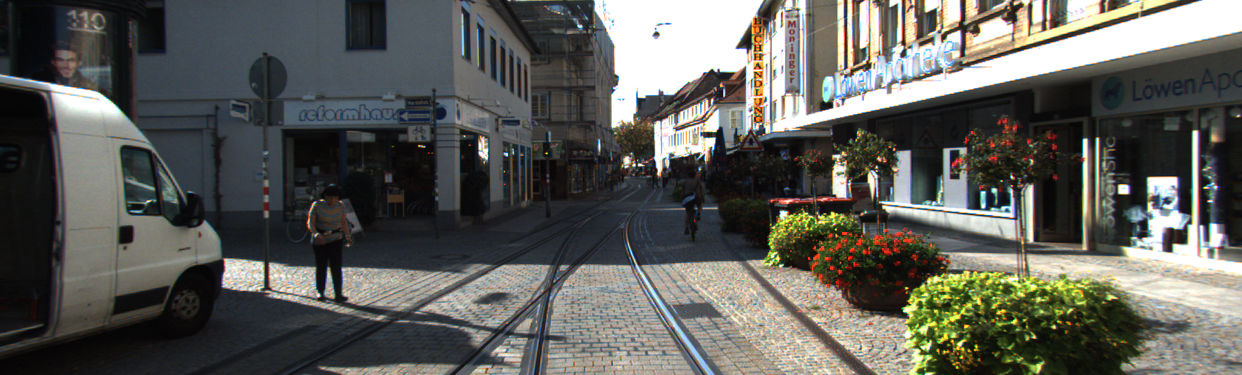
\includegraphics[width=\textwidth]{images/urban.png}
		\caption{Urban scene}
	\end{minipage}
	\hfill
	\begin{minipage}[b]{0.4\textwidth}
		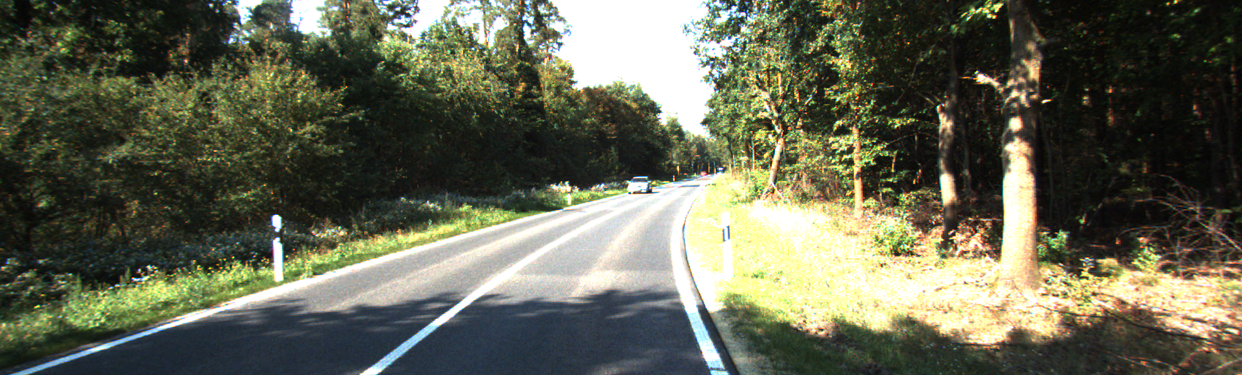
\includegraphics[width=\textwidth]{images/non_urban.png}
		\caption{Non-Urban scene}
	\end{minipage}
\end{figure}


\subsection{Image Context Detection}

Images provide a rich representation of a scene that can be exploited through image segmentation. Various image segmentation models have been developed to break down images into coherent regions.Semantic segmentation involves classifying these regions into various classes on a pixel level. 
Classic computer vision techniques for semantic segmentation utilised Texton Forests\cite{shotton2008semantic} and Random Forest classifiers \cite{shotton2011real}, however, deep learning techniques have overtaken them in terms of performance. 
Developed by Google,  Deeplab-V3 is one of the best performing open-source models on the Cityscapes semantic segmentation benchmark table. 

\subsection*{Classifying Semantic Histograms}
Using the Deeplab-V3 network, I performed semantic segmentation on the classified images. For each image, I created a semantic histogram containing the number of pixels in each semantic class as seen in figure \ref{fig:sem_hist}. By matching these histograms with the context label of the image, I was able to train a Support Vector Machine(SVM) to classify an image. Different linear and radial basis functions were tested on the SVM to see what function would perform best.

\begin{figure}[h]%
	\centering
	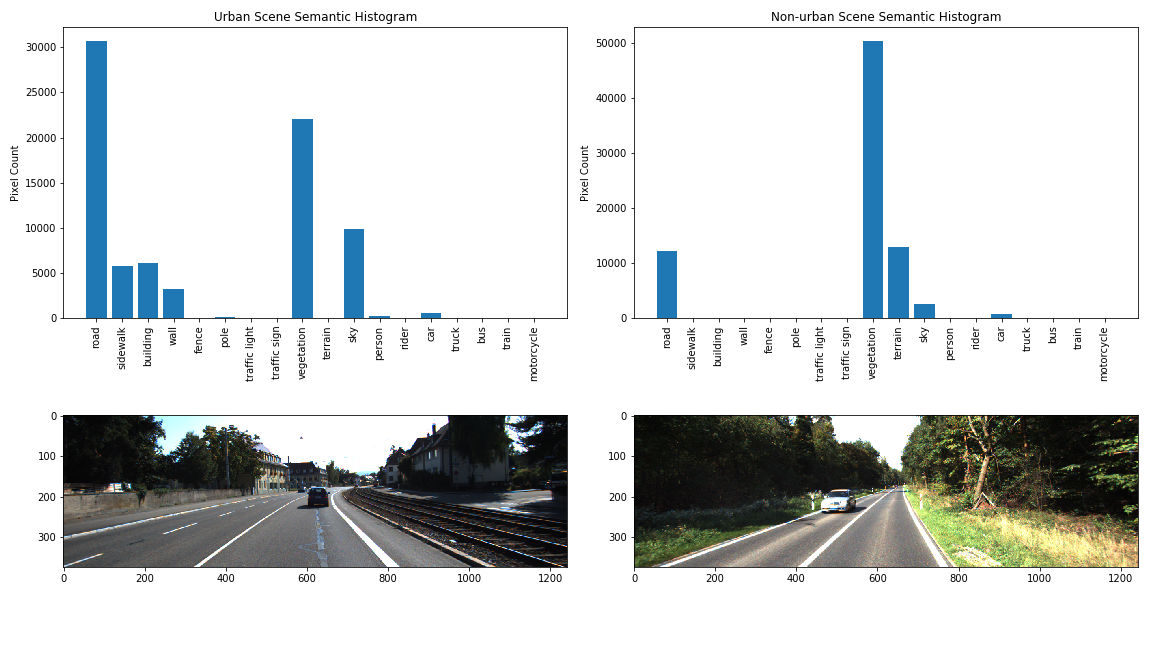
\includegraphics[width=\linewidth]{images/semantic_hist.png}%
	\caption{Semantic Histograms}%
	\label{fig:sem_hist}%
\end{figure}


\subsection{PointCloud Context Detection}
As compared to point clouds from RGB-D or stereo cameras, point clouds from LiDAR lack rich features. This is due to the sparse nature of the point clouds and as a result, the resulting representation tends to have a large number of 'holes'. Despite the availability of point clouds segmentation models, there are no datasets with annotations of outdoor scenes such as Cityscapes. As such using semantic histograms to characterise scene contexts in this case would not be suitable.
A different approach was therefore used by first detecting the key points in the cloud, extracting and classifying features from them and later on matching these features in other point clouds.  

\begin{enumerate}
	\item \textbf{Keypoint extraction} \\ 
	Similar to classic image processing, key points are salient points that are not affected by any form of transformation or distortion. As such, they are distinctive and repeatable in different points-of-view. 
	Currently, only a few 3D keypoint detectors have been proposed. These include Intrinsic Shape Signatures(ISS)\cite{}, NARF\cite{} and Uniform Sampling\cite{} of point clouds in voxels( similar to VoxelNet's).
	
	\item \textbf{Feature description} \\ 
	Signature of Histogram of Orientations
	
	
	\item \textbf{Feature Matching} \\
		

\end{enumerate}




\subsection{Implementation Issues} 

Despite being able to visually classify a large number of images, some images were difficult to classify as they exhibited characteristics from both contexts. Furthermore, due to the fact that the images was not contiguous , I was unable to infer their context by examining preceding image frames. As such, this affected the performance of both classifiers. 
\begin{figure}%
	\centering
	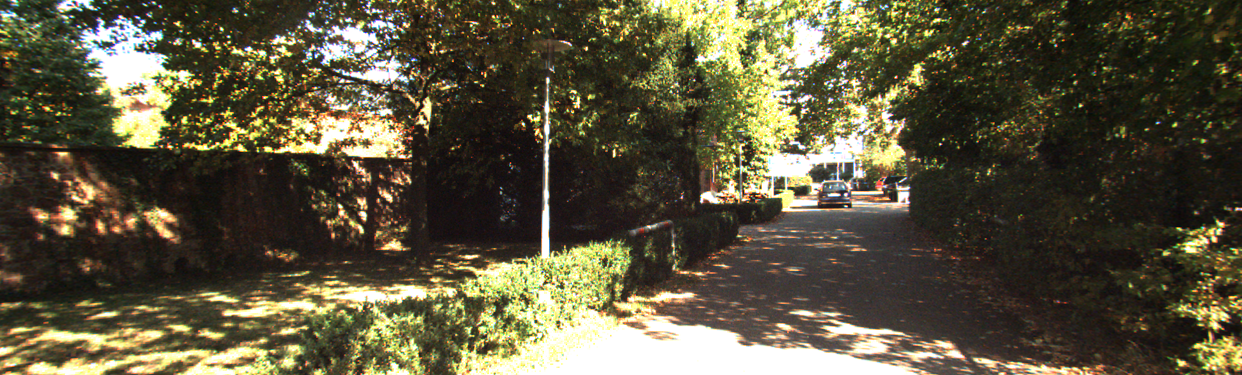
\includegraphics[width=5cm]{images/ambiguous.png}%
	\caption{Ambiguous scene}%
	\label{fig:ambiguous}%
\end{figure}

\section{ Do Some Object Detection Methods work better in Different Contexts?}

Having been able to successfully classify and create a dataset of urban and non-urban images, the next step was evaluating how a LiDAR based and image+LiDAR based object detection model would perform in different contexts. For this task,the state-of-the-art VoxelNet(LiDAR only) and AVOD(LiDAR+image) proved to be the most suitable candidates. This was influenced by the fact that they both have similar inference times, and both were open-source with the only exception being that the VoxelNet implementation was unnoficial\footnote{Had similar evaluation results as the unreleased original on KITTI benchmark.}. Both of these models were written in Python and run on the TensorFlow Deep Learning Framework.

\subsection{VoxelNet}
VoxelNet is an end to end point cloud based 3D object detection network that was released in November 2017 by leading researchers at Apple Inc. This network was one of the top performing LiDAR only models on the KITTI benchmark. However, the code was never released and only unnoficial implementations are currently available online.
\subsubsection{Architecture Overview}
VoxelNet is composed of three fundamental blocks. 
\begin{enumerate}
	\item \textbf{Voxel Feature Encoding Layer} \\ 
	
	\item \textbf{Convolutional Middle Layers} \\ 
	\item \textbf{Region Proposal Network} \\ 
\end{enumerate}

\subsubsection{Implementation Details}





\subsection{AVOD}


\subsubsection{Architecture Overview}



\subsubsection{Implementation Details}











\subsection{Evaluating with KITTI Dataset}


\



\subsection{Is VoxelNet Performance Valid for Different Datasets?}
To validate the VoxelNet model, I used the Smart Internet Lab dataset that was obtained from a LiDAR positioned on a stationary car. 
\subsubsection*{Preprocessing}
Before using the data on VoxelNet, the data had to be preprocessed to the necessary input format. 
VoxelNet only required four input fields, \textbf{XYZ values} and \textbf{reflectance} of the points, whereas the dataset was in the form of network capture files(.pcap ). To convert them into this format, I exported the capture filed into CSV format for each of the frames. This was done  in VeloView using the CSV export function. The result was a CSV file with 13 fields as seen in figure \ref{fig:sildata}

\begin{figure}[h]
	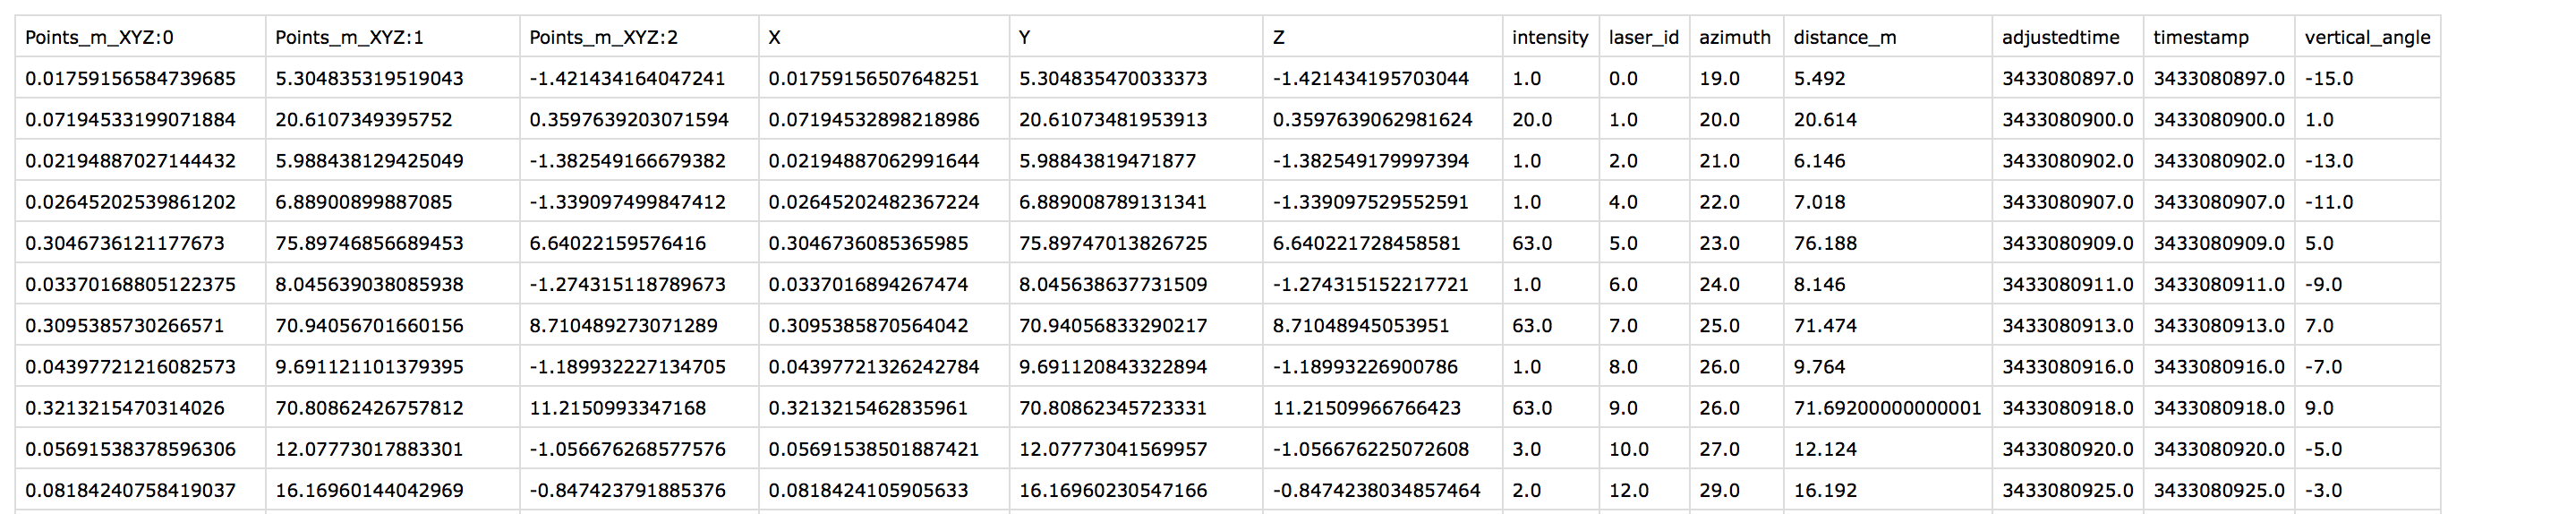
\includegraphics[width=\linewidth]{images/sildata.png}
	\caption{Smart Internet Lab Frame CSV}
	\label{fig:sildata}
\end{figure}

Out of the 13 fields, I extracted the XYZ values and intensity(reflectance) of the points and saved them as Numpy binary files. This resulted in a smaller file sizes(from around 4MB to 70KB) that are also quicker to read than normal CSV files.

\begin{figure}[h]
	\centering
	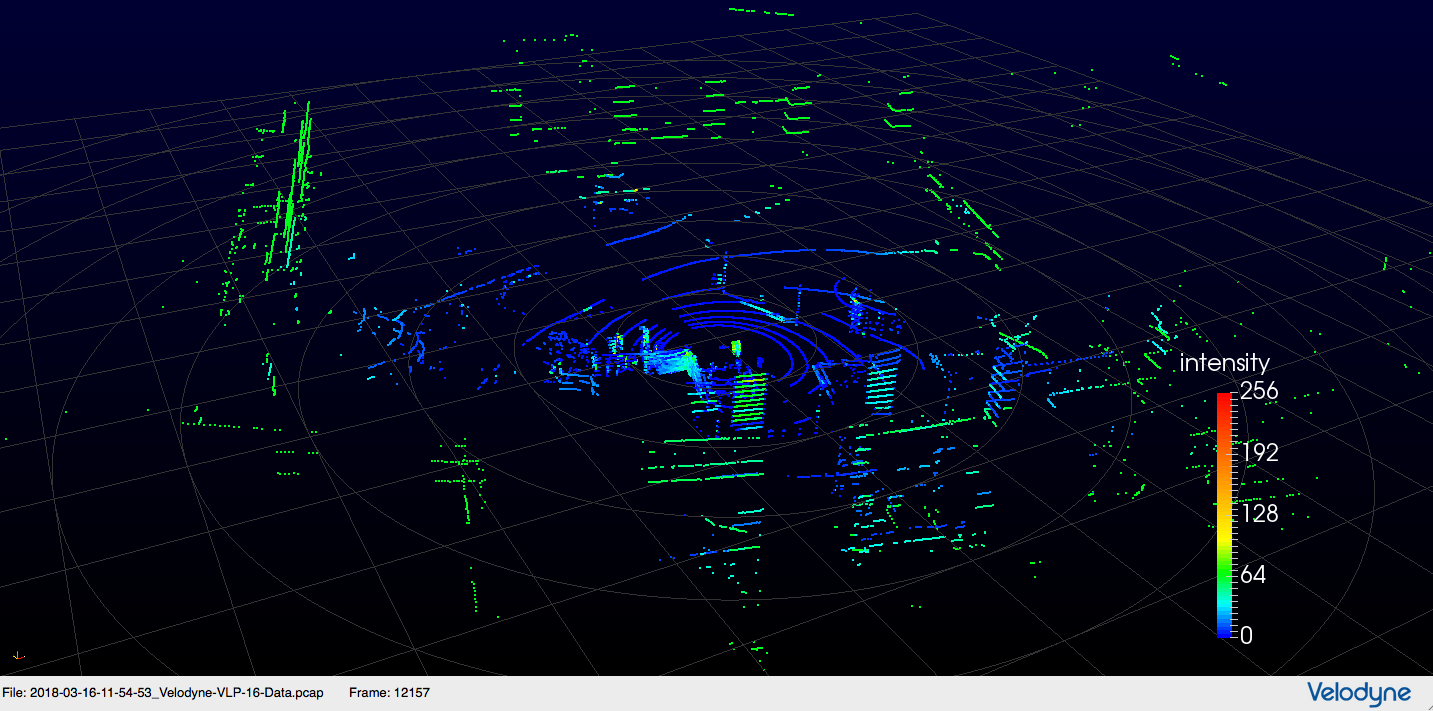
\includegraphics[width=\linewidth]{images/sil.png}
	\caption{Veloview Frame of Smart Internet Lab data}
	\label{fig:sil}
\end{figure}


Finally, I modified VoxelNet's configuration file to include the specifications for the VLP-16 LiDAR sensor. This was essential as the network was initially trained on KITTI point clouds that were obtained from a Velodyne HDL-64E with different specifications as seen in table \ref{vlp-hdl}. These specifications are necessary for manipulating the point clouds and therefore directly affect the performance of the network. The modified entries were the angular and vertical resolution, maximum and minimum XYZ values and the height of the VLP-16 LiDAR sensor on the vehicle. Given that there was no image data for visualisation, the image size in the configuration file was set to 0 to prevent unnecessary tensor memory allocation for images. 

\begin{table}[H]
	\centering
	\resizebox{\textwidth}{!}{%
		\begin{tabular}{|l|l|l|l|l|l|l|}
			\hline
			\textbf{LiDAR}       & \textbf{Hor FOV} & \textbf{Ver FOV} & \textbf{Range} & \textbf{Angular Resolution} & \textbf{Points/second}          & \textbf{Channels} \\ \hline
			\textit{\textbf{HDL-64E}} & 360\degree                    & 26.9\degree                 & 120m           & $\sim$0.4\degree                          & $\sim$2.2 Million                   & 64                \\ \hline
			\textit{\textbf{VLP-16}}  & 360\degree                    & $\pm$ 15\degree                 & 100m           & 0.1\degree                                & 600,000                             & 16                \\ \hline
		\end{tabular}
	}
	
	\caption{Velodyne HDL-64E and VLP-16 Specifications.}
	\label{vlp-hdl}
\end{table}

\subsubsection*{Annotating Ground Truth Labels}
The SIL dataset did not contain any ground truth labels for the point clouds as compared to the KITTI dataset. As a result, there was no metric to assess the performance of the network. To prevent this, objects from the dataset needed to be annotated to obtain some ground truth bounding boxes. 

\noindent
\textbf{L-CAS Annotation Tool} \\ 
Developed by the Lincoln Centre for Autonomous Systems Research, this tool provides a semi-automatic labelling function that clusters and highlight regions of interest that may contain objects. The user can then label them depending on the object class such as car, cyclist, pedestrian. The result is then stored in a file containing the objects and their positions in the point cloud. 
To use this tool, the .pcap capture files were converted into .pcd format using the 
ROS velodyne point cloud package\footnote{See listing \ref{lst:ros}}. 

\begin{figure}[h]
	
	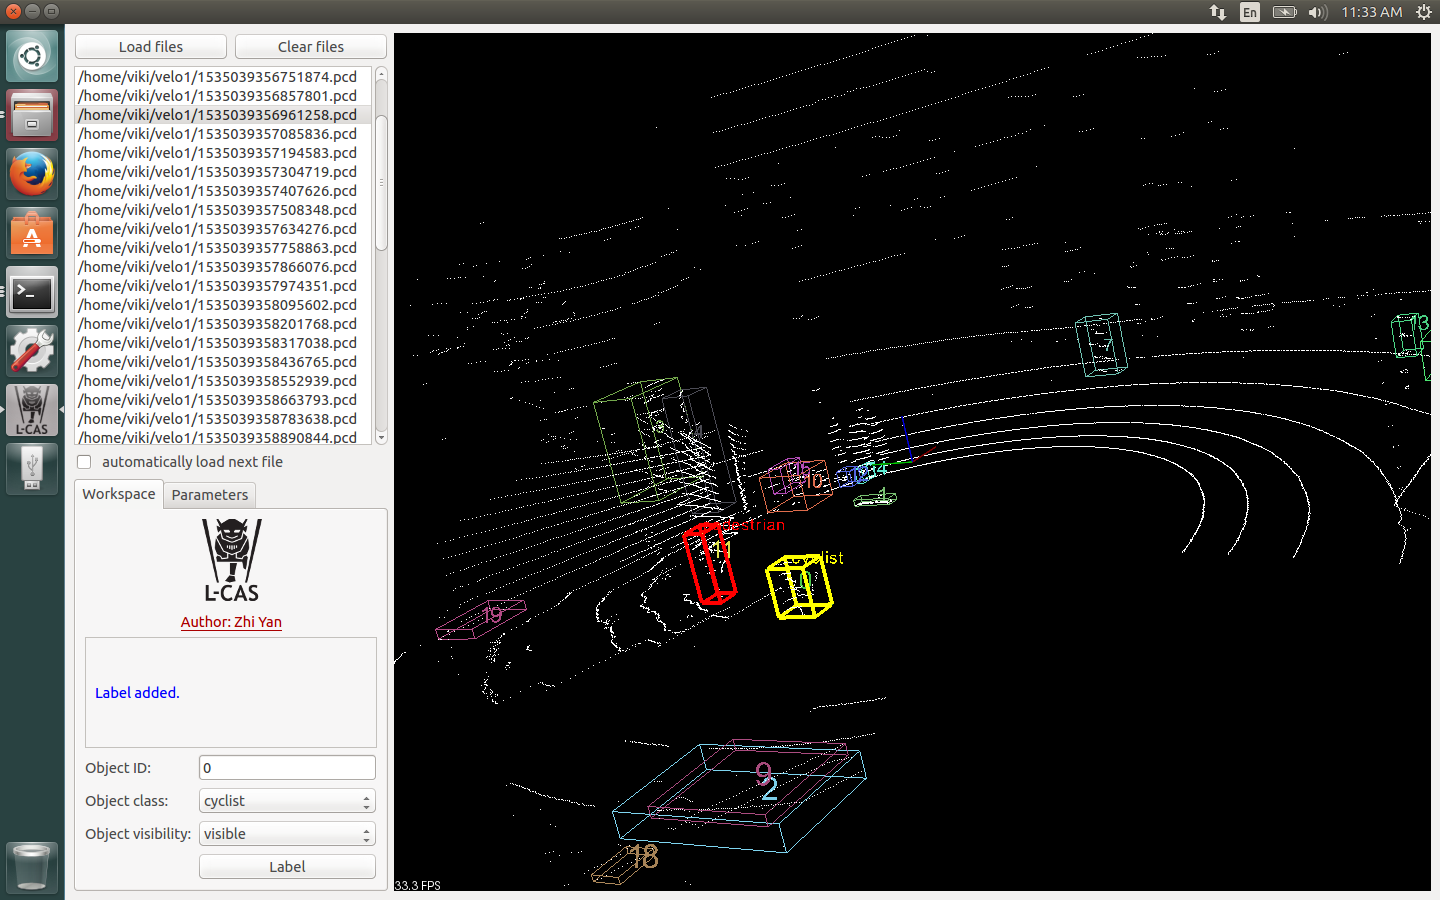
\includegraphics[width=\linewidth]{images/annot.png}
	\caption{L-CAS Annotation Tool}
	\label{fig:annot}
\end{figure}


